\documentclass[a4paper]{itat}
%\usepackage{slovak}

\usepackage[cp1250]{inputenc}  % or [cp1250], or [latin2], or whatever
                               % suitable for your system

\usepackage{graphicx}
\usepackage{url}


\begin{document}
\begin{twocolumn}
%%%%%%%%%%%%%%%%%%%%%%%%%%%%%%%%%%%%%%%%%%%%%%%%%%%%%%%%%%%%%%%%%%%%%%%%%%%%%%%%%%%%%%%%%%


\title{Web Information Extraction Systems for Web Semantization}

\titlerunning{WIE Systems for Web Semantization}

\author{Jan Dedek}
\authorrunning{Jan Dedek}

\institute{Department of software engineering, Faculty of Mathematics and Physics\\
Charles University in Prague, Czech Republic\\
\email{dedek@ksi.mff.cuni.cz}
}

\maketitle              % typeset the title of the contribution

\begin{abstract}
In this paper we present a survey of web information extraction systems and semantic annotation platforms. The survey is concentrated on the problem of employment of these tools in the process of web semantization. We compare the approaches with our own solutions and propose some future directions in the development of the web semantization idea.
\end{abstract}

%%%%%%%%%%%%%%%%%%%%%%%%%%%%%%%%%%%%%%%%%%%%%%%%%%%%%%%%%%%%%%%%%%%%%%%%%%%%%%%%%%%%%%%%%%
\section{Introduction} \label{sec:intro}


There exist many extraction tools that can process web pages like this. Most complete recent survey can be found in \cite{biblio:Chang2006} and also in \cite{biblio:WebDataMining}.  We come with similar but also different solution divided into domain dependent and domain independent phases. See below for details.

\subsection{Web Semantization}
\subsection{Use of the Semantic Data}

\begin{figure}
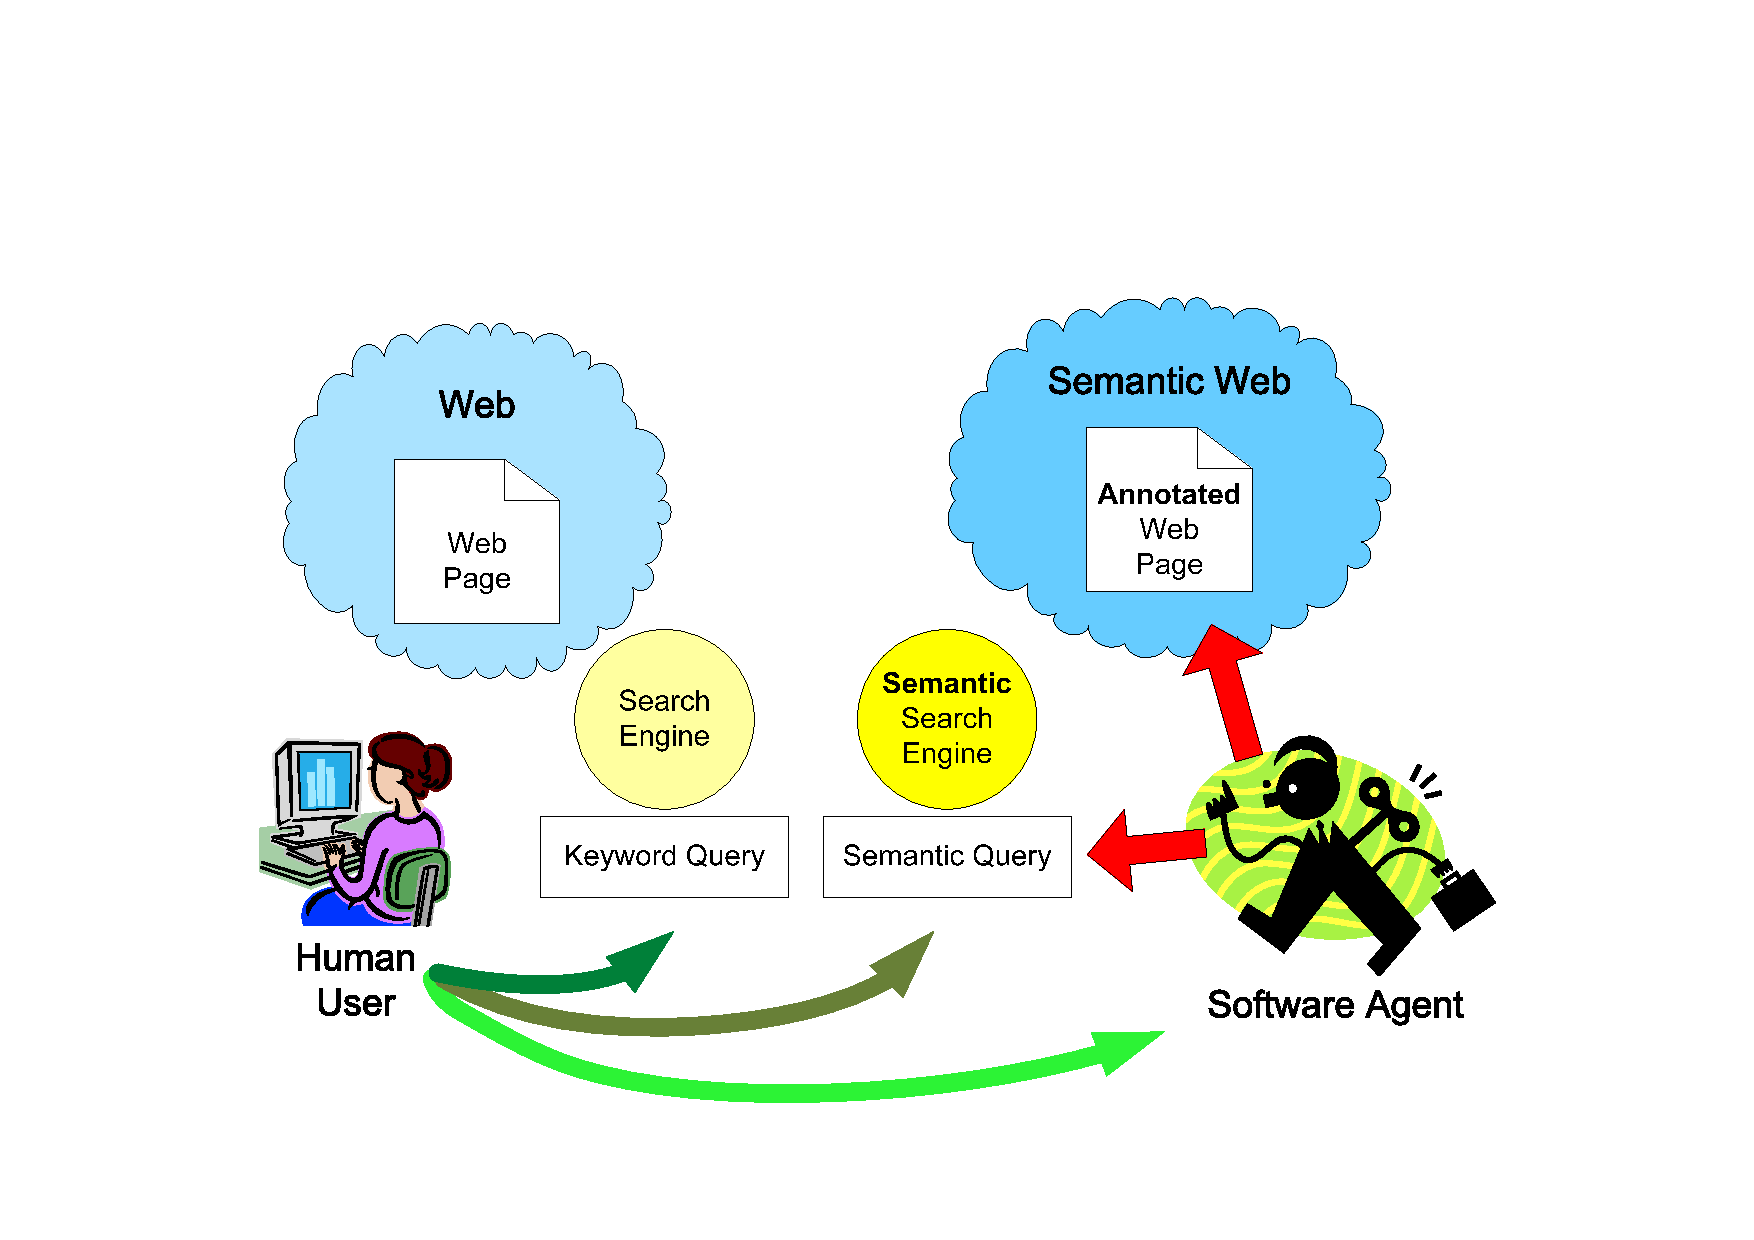
\includegraphics[width=\hsize]{img/SemanticWeb}
\caption{Exploitation of the semantic data}
\label{img:prologFacts}
\end{figure}


%%%%%%%%%%%%%%%%%%%%%%%%%%%%%%%%%%%%%%%%%%%%%%%%%%%%%%%%%%%%%%%%%%%%%%%%%%%%%%%%%%%%%%%%%%
\section{Web Information Extraction} \label{sec:WIE}

\subsection{Domain Specific}
\subsection{Form Specific}


%%%%%%%%%%%%%%%%%%%%%%%%%%%%%%%%%%%%%%%%%%%%%%%%%%%%%%%%%%%%%%%%%%%%%%%%%%%%%%%%%%%%%%%%%%
\section{Information Extraction Based on Linguistics} \label{sec:LingIE}
\subsection{Tasks of Information Extraction}
There are classical tasks of text preprocessing and linguistic analysis like 
\begin{description}
	\item[text extraction] -- e.g from HTML, PDF or DOC,
	\item[tokenization] -- detection of words, spaces, punctuations, etc.,
	\item[segmentation] -- sentence and paragraph detection,
	\item[POS tagging] -- part of speech assignment, often including lemmatization and morphological analysis,
	\item[syntactic analysis] (often called linguistic \emph{parsing}) -- assignment of the grammatical structure to given sentence with respect to given linguistic formalism (e.g. formal grammar),
	\item[coreference resolution] (or \emph{anaphora resolution}) -- resolving what a pronoun, or a noun phrase refers to. These references often cross boundaries of a single sentence.
\end{description}

Besides these classical general applicable tasks, there are further well defined tasks, which are more closely related to the information extraction. These tasks are domain dependent. These tasks were widely developed in the MUC-6 conference 1995 \cite{biblio:MUC6} and considered as semantic evaluation in the first place. These information extraction tasks are:

\begin{description}
	\item[Named Entity Recognition:] This task recognizes and classifies named entities such as persons, locations, date or time expression, or measuring units. More complex patterns may also be recognized as structured entities such as addresses.
	\item[Template Element Construction:] Populates templates describing entities with extracted
roles (or attributes) about one single entity. This task is often performed stepwise sentence by sentence, which results in a huge set of partially filled templates.
	\item[Template Relation Construction:] As each template describes information about one single entity, this tasks identifies semantic relations between entities.
	\item[Template Unification:] Merges multiple elementary templates that are filled with information about identical entities.
	\item[Scenario Template Production:] Fits the results of Template Element Construction and Template Relation Construction into templates describing pre-specified event scenarios (pre-specified ``queries on the extracted data'').
\end{description}

Appelt and Israel \cite{biblio:Appelt-Israel} wrote an excellent tutorial summarizing these traditional IE tasks and systems built on them.


  

\subsection{Information Extraction Benchmarks}

There are several conferences and events concentrated on the support of automatic machine processing and understanding of human language in text form. Different research topics as text (or information) retrieval\footnote{e.g. Text REtrieval Conference (TREC)\\ \url{http://trec.nist.gov/}}, text summarization \footnote{e.g. Document Understanding Conferences\\ \url{http://duc.nist.gov/}} are involved.

On the filed of information extraction, we have to mention the long tradition of the Message Understanding Conference\footnote{Briefly summarized in \url{http://en.wikipedia.org/wiki/Message_Understanding_Conference}.} \cite{biblio:MUC6} starting in 1987. In 1999 the event of \emph{Automatic Content Extraction (ACE) Evaluation}\footnote{\url{http://www.itl.nist.gov/iad/mig/tests/ace/}} started, which is becoming a track in the Text Analysis Conference (TAC)\footnote{\url{http://www.nist.gov/tac}} this year (in 2009).

All these events prepare several specialized datasets together with information extraction tasks and play an important role of information extraction benchmarks. 

%%%%%%%%%%%%%%%%%%%%%%%%%%%%%%%%%%%%%%%%%%%%%%%%%%%%%%%%%%%%%%%%%%%%%%%%%%%%%%%%%%%%%%%%%%
\section{Our Solutions} \label{sec:OurSolutins}
\subsection{Extraction Based on Structural Similarity}
\subsection{Linguistic Information Extraction}
This solution is directed to extraction of information which is closely connected with the meaning of text or meaning of a sentence. 

Difficult task.

Problematic usage of extracted data.


%%%%%%%%%%%%%%%%%%%%%%%%%%%%%%%%%%%%%%%%%%%%%%%%%%%%%%%%%%%%%%%%%%%%%%%%%%%%%%%%%%%%%%%%%%
\section{The Web Semantization Setting} \label{sec:SemantizationSetting}

\begin{figure*}
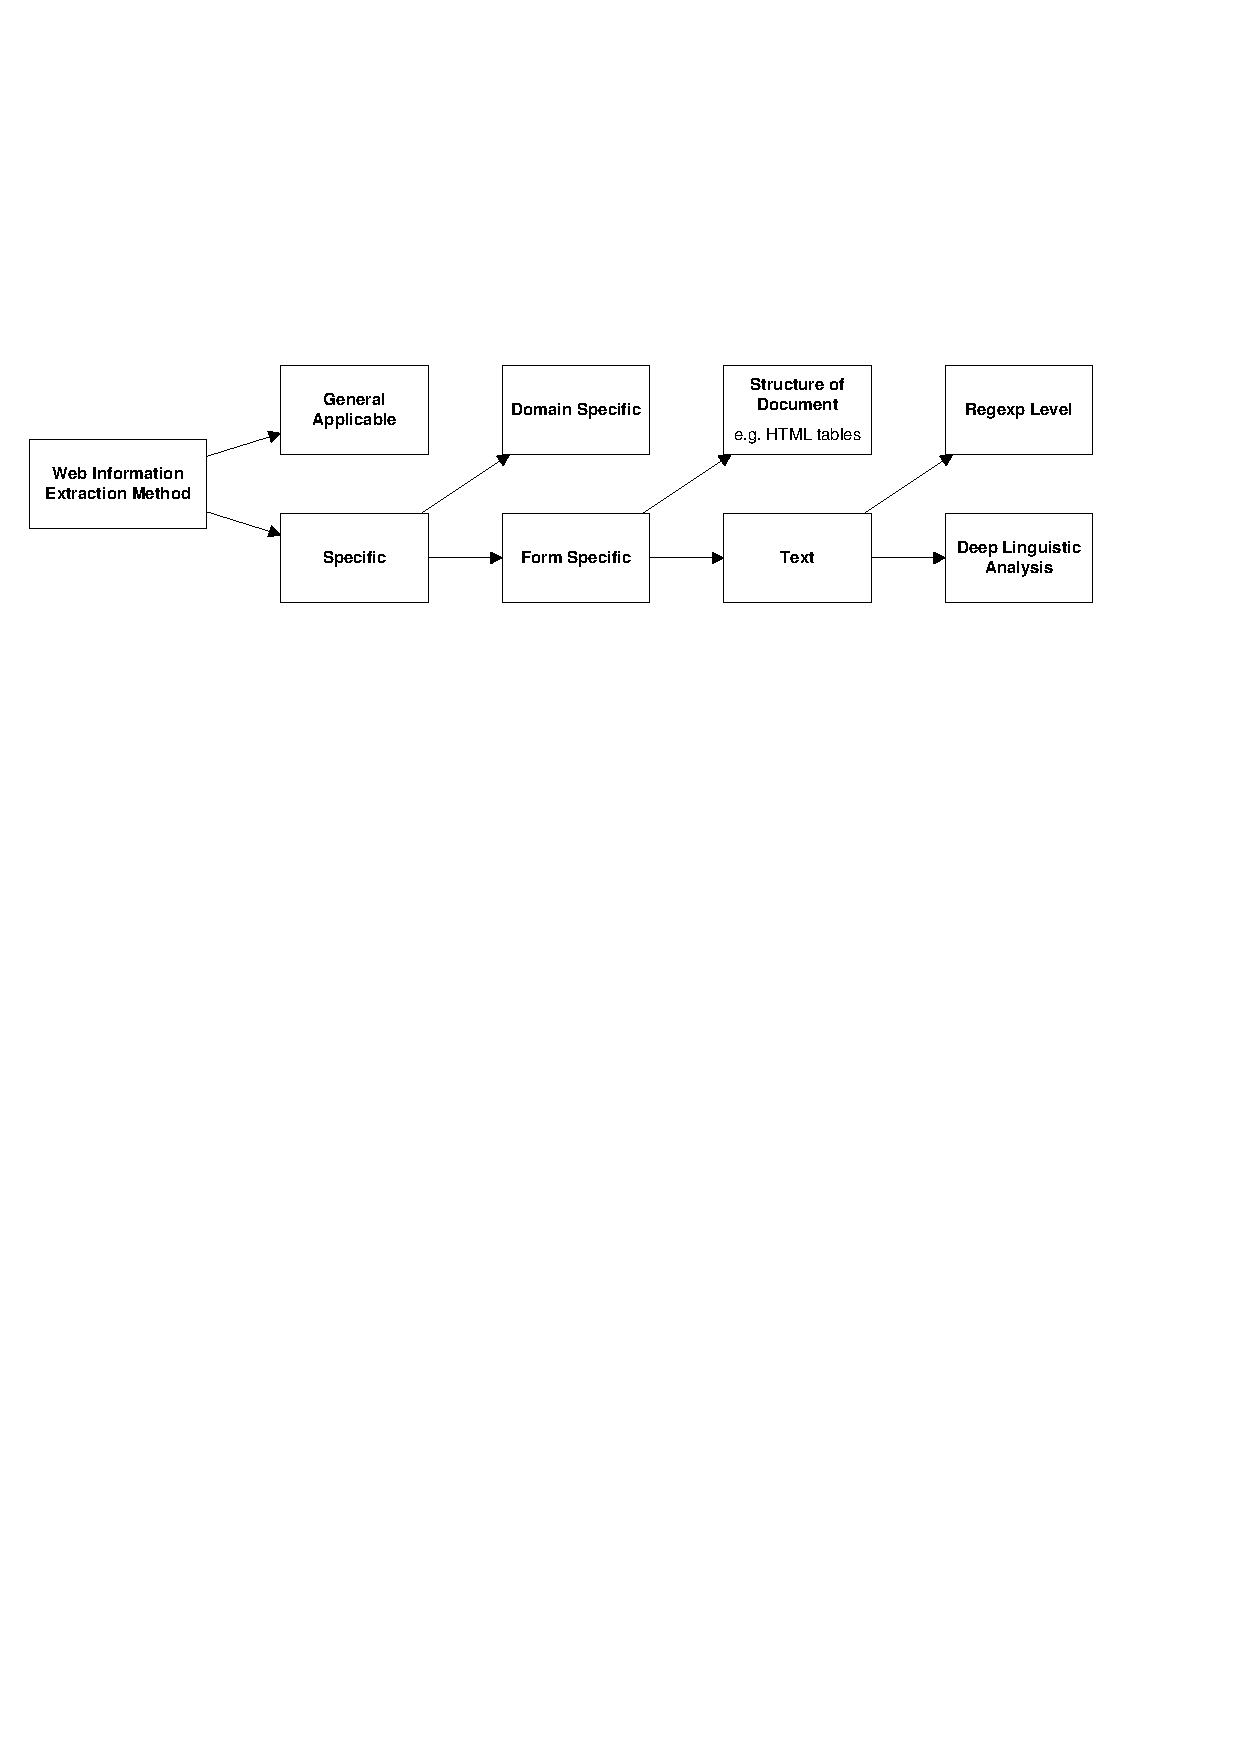
\includegraphics[width=\hsize]{img/extraction_method}
\caption{Division of extraction methods}
\label{img:extraction_method}
\end{figure*}

\begin{figure}
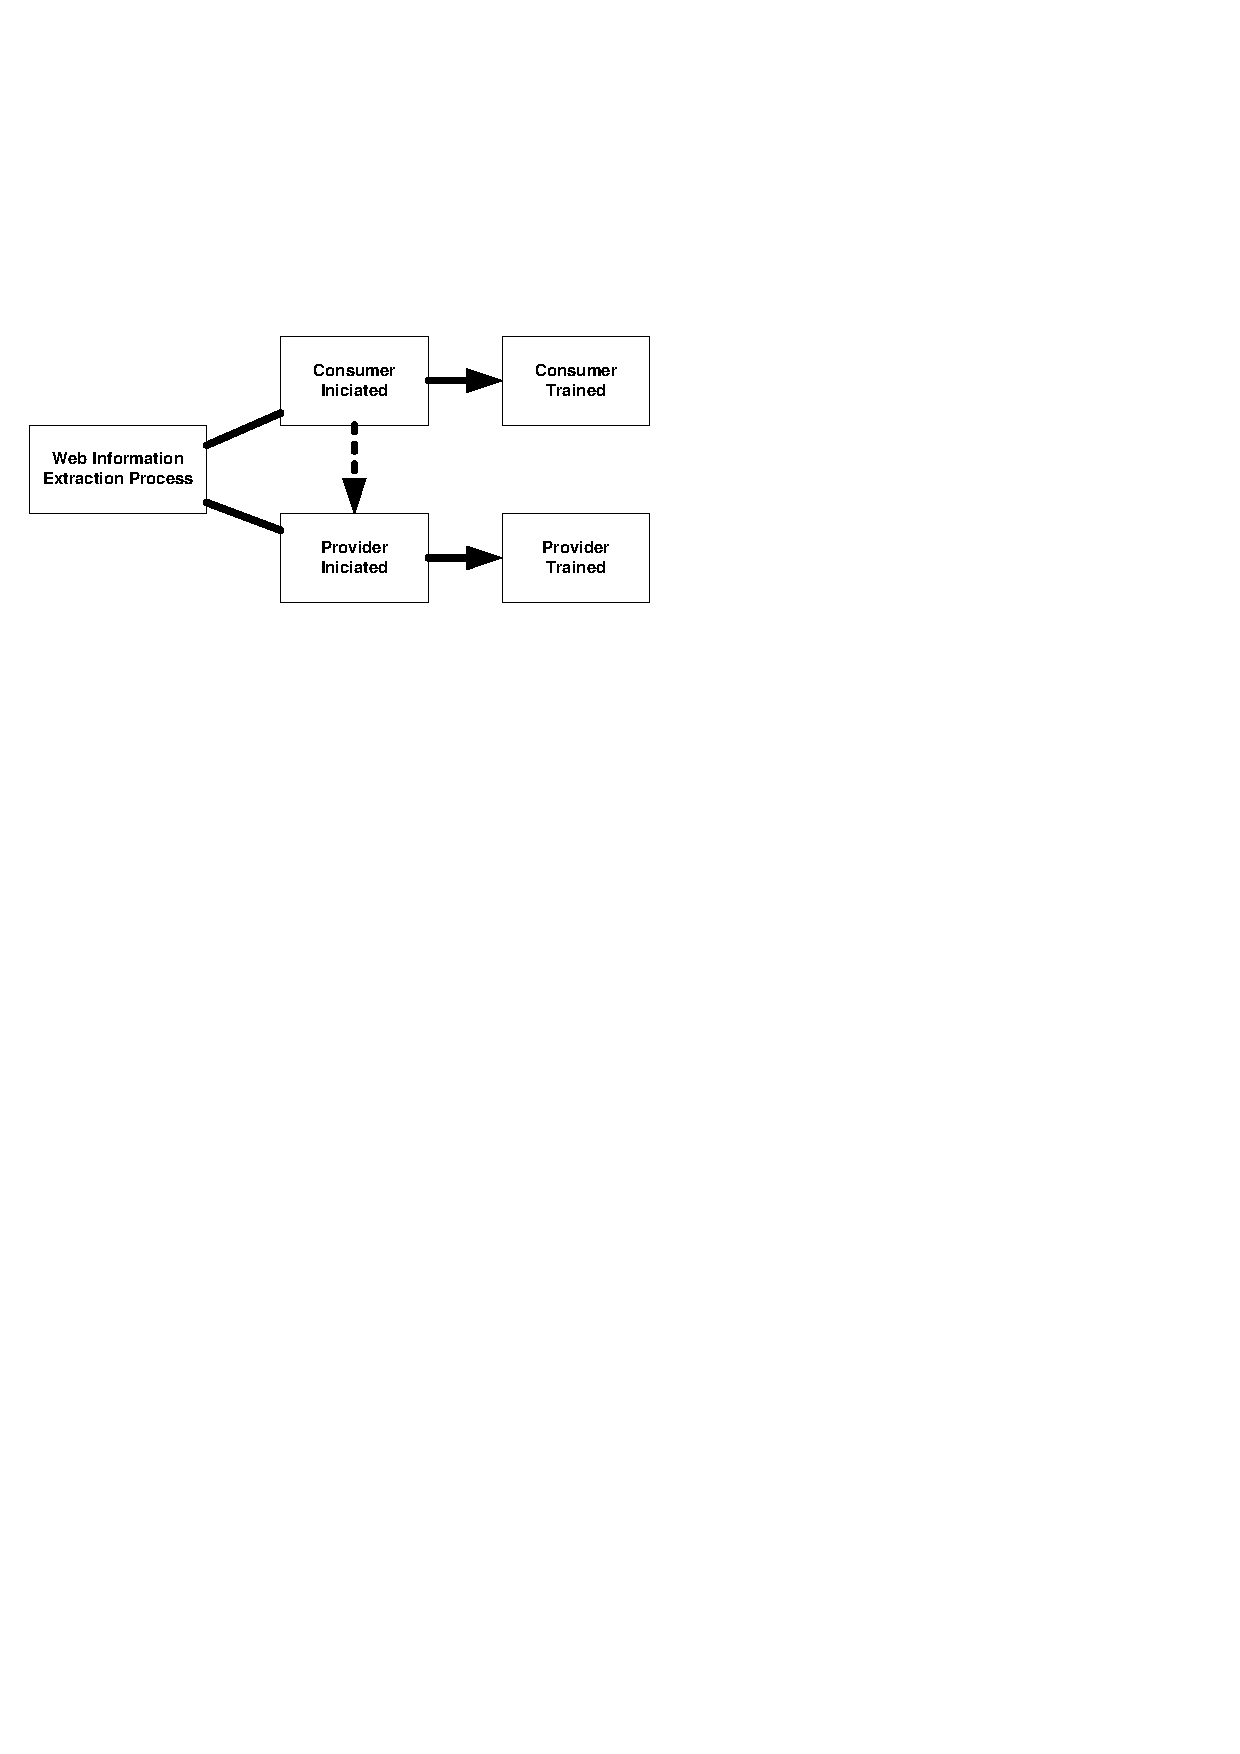
\includegraphics[width=\hsize]{img/extraction_proces_and_user}
\caption{User view on the extraction process}
\label{img:extraction_proces_and_user}
\end{figure}


%%%%%%%%%%%%%%%%%%%%%%%%%%%%%%%%%%%%%%%%%%%%%%%%%%%%%%%%%%%%%%%%%%%%%%%%%%%%%%%%%%%%%%%%%%
\section{Conclusion and Future Work} \label{sec:conlusion}


\section*{Acknowledgments}
This work was partially supported by Czech projects 1ET100300517, 201/09/H057 GA�R %Czech Science Foundation
and MSM-0021620838.

%%%%%%%%%%%%%%%%%%%%%%%%%%%%%%%%%%%%%%%%%%%%%%%%%%%%%%%%%%%%%%%%%%%%%%%%%%%%%%%%%%%%%%%%%%
\bibliographystyle{plain}
\bibliography{Dedek_ITAT}


%%%%%%%%%%%%%%%%%%%%%%%%%%%%%%%%%%%%%%%%%%%%%%%%%%%%%%%%%%%%%%%%%%%%%%%%%%%%%%%%%%%%%%%%%%
\end{twocolumn}
\end{document}
